\documentclass[pdf,aspectratio=169]{beamer}
\usepackage[]{hyperref,graphicx,siunitx,lmodern,booktabs,tikz,tensor}
\usepackage{pdfpc-commands}

\usepackage[mode=buildnew]{standalone}
\mode<presentation>{\usetheme{Astro}}

\graphicspath{ {../Images/} }

\sisetup{per-mode=symbol}
\usetikzlibrary{calc,intersections, decorations.pathmorphing,shadings}
\tikzstyle{proton}=[circle, minimum size = 7mm, ball color=red, black,transform shape]
\tikzstyle{neutron}=[circle, minimum size=7mm, ball color=gray, black, transform shape]
\tikzstyle{gammaray}=[ultra thick, -latex, decorate, decoration={snake, post length=3mm}]
\tikzstyle{image}=[inner sep=0pt, outer sep=0pt, anchor=south west]


%preamble
\title{Lifestyles of the Low Mass and Famous}
\date{November 5, 2018}
\author{Jed Rembold}

\begin{document}
\renewcommand*{\theenumi}{\Alph{enumi}}

\begin{frame}{Announcements}
  \begin{itemize}
	  \item Webwork due on Wednesday
	  \item Keep in mind: Poor test scores with high homework scores are recoverable. Poor test scores with poor homework scores will definitely hurt.
	  \item Lab Group A meeting tonight!
	  \item Test 3 one week from Friday
	  \item Polling: \url{rembold-class.ddns.net}
  \end{itemize}
\end{frame}

\begin{frame}{APOD!}
	\begin{center}
		\includegraphics[width=0.5\textwidth]{APOD_M5.png}
	\end{center}
\end{frame}

\begin{frame}{Let's Review\ldots}
  We can determine the age of a star cluster by:
  \begin{enumerate}
	\item Estimating the number of stars in the cluster
	\item Finding the average luminosity of its stars
	\item Looking at the average temperature of the cluster
	\item \alert<2>{Determining where it leaves the main sequence}
  \end{enumerate}
\end{frame}

\begin{frame}{Making a Star: Gather Your Ingredients}
	\begin{columns}
		\column{0.5\textwidth}
		  \begin{itemize}
			  \item Ch 21.1 and 21.2
			\item Stars are formed in giant molecular clouds
			  \begin{itemize}
				\item Dense, cold, dusty regions of interstellar space
				\item ``Dense'' is relative here\ldots
			  \end{itemize}
		  \end{itemize}
		
		\column{0.5\textwidth}
		  \begin{center}
			\includegraphics[width=.9\textwidth]{ch12_dark_cloud.jpg}
		  \end{center}
		
	\end{columns}
\end{frame}

%\begin{frame}{Easiest to See in Infrared}
  %\begin{center}
	%\begin{tikzpicture}
	  %\node[image] at (0,0) {\includegraphics[width=7cm]{ch12_Cloud1.png}};
	  %\node<2>[image, opacity=0.5] at (0,0) {\includegraphics[width=7cm]{ch12_Cloud2.png}};
	  %\node<3>[image, opacity=1.0] at (0,0) {\includegraphics[width=7cm]{ch12_Cloud2.png}};
	%\end{tikzpicture}
  %\end{center}
%\end{frame}

\begin{frame}{Bring it in\ldots}
  \begin{itemize}
	\item Need gravity to be greater than any internal gas pressure
	  \begin{itemize}
		\item Easiest with dense, cold regions
		\item Hence the molecular clouds
	  \end{itemize}
	\item Densest regions attract the most gas
	  \begin{itemize}
		\item Breaks a cloud up into various smaller clouds
		\item Each smaller, dense cloud can continue to contract to become a protostar
	  \end{itemize}
  \end{itemize}
  \begin{center}
	\includegraphics[width=7.5cm]{ch12_orion_infrared.jpg}
  \end{center}
\end{frame}

\begin{frame}{Protostars}
  \begin{columns}
	\column{.5\textwidth}
	\begin{itemize}
	  \item Molecular cloud moves towards random regions of density
	  \item Gravity further isolates and condenses dense regions
	  \item The resulting cloud fragment is generally called a \alert{protostar}
		\begin{itemize}
		  \item Not yet hot enough to start nuclear fusion!
		  \item Can still be bright due to the energy loss of inward moving gas
		\end{itemize}
	\end{itemize}
	\column{.5\textwidth}
	\begin{center}
	  \includegraphics[width=\textwidth]{ch13_protostar.jpg}
	\end{center}
  \end{columns}
\end{frame}

\fullFrameMovie{../Videos/protostar_birth.ogv}{../Videos/protostar_birth.png}

\begin{frame}{Yo Momma So Fat\ldots}
  \begin{itemize}
	\item For a cloud of some density and temperature, how much mass do we need to ``win'' and collapse to form protostars?
	  \[M_{min} = 18 M_{\odot}\sqrt{\frac{T^3}{n}}\]
	  where
	  \begin{itemize}
		\item $T$ is the temperature of the gas cloud
		\item $n$ is the gas density in terms of particles per cubic centimeter
		\item $M_{min}$ is the minimum mass needed for the cloud to collapse and start creating stars
		\item $M_\odot$ is the mass of the Sun
	  \end{itemize}
  \end{itemize}
\end{frame}

\begin{frame}{Example}
  \begin{example}
	Suppose I observed a massive molecular cloud,  with the below properties:
	\begin{itemize}
	  \item $T=\SI{25}{\kelvin}$
	  \item $n = \SI{500}{particles\per\centi\meter^3}$
	  \item $M = 75 M_{\odot}$
	\end{itemize}
	Should I expect this molecular cloud to collapse into protostars?
  \end{example}
  \begin{alertblock}<2>{NO!}
	$M_{min} = 100.62 M_\odot$
  \end{alertblock}
\end{frame}

\begin{frame}{Jets!}
  \begin{itemize}
	\item Life as a protostar is often violent!
	\item Rapid rotations lead to disk flattening
	\item We commonly see jets emanating from the poles
	  \begin{itemize}
		\item Help shed angular momentum?
		\item Influenced by strong magnetic fields
	  \end{itemize}
  \end{itemize}
  \begin{center}
	\includegraphics<1>[width=\textwidth]{ch13_Jets.jpg}
	\includegraphics<2>[width=.9\textwidth]{ch21_jets2.png}
  \end{center}
\end{frame}


\begin{frame}{Onward toward the Main Sequence!}
  \begin{itemize}
	\item More massive stars do everything faster!
	\item Protostar lifetimes
	  \begin{itemize}
		\item O or B type: a million years or so
		\item G type: 30 million years
		\item M type: $>$100 million years
	  \end{itemize}
	\item Makes it possible for some massive stars to ignite, shine, run out of fuel and die before a smaller baby star even starts fusion!
  \end{itemize}
  \begin{center}
	\begin{tikzpicture}
	  \node[anchor=south west, inner sep=0pt, outer sep=0pt] at (0,0) {\includegraphics[width=2.3cm]{ch13_oldman.pdf}};
	  \node[anchor=south west, inner sep=0pt, outer sep=0pt] at (3,5mm) {\inlineMovie{../Videos/JackJack.ogv}{../Videos/JackJack.png}{width=6cm}};
	\end{tikzpicture}
  \end{center}
\end{frame}

\begin{frame}{What's being born?}
  \begin{columns}
	\column{.5\textwidth}
	\begin{itemize}
	  \item High mass stars are rare
	  \item Low mass stars are much more common
	\end{itemize}
	\begin{center}
	  \begin{tikzpicture}[scale=.7, transform shape]
		\node[inner sep=0pt, outer sep=0pt, anchor=south west] at (0,0) {\includegraphics[width=8cm]{ch13_mass_distribution.jpg}};
		%\draw[orange] (0,0) grid (6,4);
		\node at (6mm, -2mm) {0.08};
		\node at (24mm, -2mm) {0.5};
		\node at (36mm, -2mm) {2};
		\node at (50mm, -2mm) {10};
		\node at (74mm, -2mm) {150};
		\node at (4,-8mm) {stellar mass ($M_{\odot}$)};
		\node[rotate=90] at (-4mm, 28mm) {relative number of stars};
	  \end{tikzpicture}
	\end{center}
	\column{.5\textwidth}
	\begin{center}
	  \includegraphics[width=.65\textwidth]{ch13_starlist.jpg}
	\end{center}
  \end{columns}
\end{frame}

\begin{frame}{The Highs and Lows of Life}
  \begin{itemize}
	\item Upper limit of star mass
	  \begin{itemize}
		\item Largest observed about $150 M_\odot$
		\item May be some a bit larger
		\item Luminosity actually gets so high it starts blowing parts of the star itself away
	  \end{itemize}
	\item Lower limit
	  \begin{itemize}
		\item Need at least $0.08 M_\odot$ to ignite nuclear fusion reliably
		\item Radiate primarily in the infrared
		\item Slowly cool due to missing an energy source
		\item Called Brown Dwarfs
	  \end{itemize}
  \end{itemize}
\end{frame}

\begin{frame}{The Brown Dwarfs}
  \begin{itemize}
	\item Occupy the space between large planet and tiny star
	\item Glow reddish
	\item Without fusion to provide an energy source, why does gravity not crush them?
	  \begin{itemize}
		\item Degeneracy Pressure
	  \end{itemize}
  \end{itemize}
  \begin{center}
	\includegraphics[width=.6\textwidth]{ch13_browndwarf.jpg}
  \end{center}
\end{frame}

\begin{frame}[fragile]{Parking Lot Degeneracy Pressure}
  \begin{itemize}
	\item Pauli Exclusion Principle limits numbers of particles in certain states
	\item ``Backs up traffic'' as particles have to search and work harder to find space
  \end{itemize}
  \begin{center}
	\begin{tikzpicture}
	  \newcommand{\car}[3]{
		\begin{scope}[#3]
		  \fill[#2, rounded corners=1mm] (#1) --++(-5mm,0) --++(0,3mm) --++(2mm,0) --++(1mm,1mm) --++(4mm,0)--++(1mm,-1mm) --++(2mm,0) --++(0,-3mm) -- cycle;
		  \fill[] ($(#1)+(-3mm,0)$) circle (3pt);
		  \fill[] ($(#1)+(3mm,0)$) circle (3pt);
		\end{scope}
		}
		\draw[thick] (0,0) --+(0,4);
		\foreach \y in {0,1,2,3,4} \draw[thick] (0,\y) --+(1.5,0);
		\draw[thick] (5,0) --+(0,4);
		\foreach \y in {0,1,2,3,4} \draw[thick] (5,\y) --+(-1.5,0);

		\car{.75,.3}{green}{}
		\car{.75,2.3}{violet}{}
		\car{4.25,1.3}{orange}{}
		\car{3,4.5}{cyan}{rotate around={30:(3,4.5)}}
		\car{2.5,1}{yellow}{rotate around={90:(2.5,1)}}

		\only<2>{
		  \draw[dashed, cyan, very thick, -latex] (3,4.5)++(210:4mm) to[bend left] (.8,3.5);
		  \draw[dashed, yellow, very thick, -latex] (2.5,1.5) to[bend left] (4.2,2.5);
		}
		\only<3->{
		  \car{.75,1.3}{red}{}
		  \car{.74,3.3}{blue}{}
		  \car{4.25,.3}{violet!60!black}{}
		  \car{4.25,3.3}{green!40!black}{}
		}
		\only<4>{
		  \draw[dashed, yellow, very thick, -latex] (2.5,1.5) to[bend left] (4.2,2.5);
		  \draw[dashed, cyan, very thick, -latex] (2.5,4.4) to[bend right] (2.5,3) node[below] {\LARGE?};
		}

	\end{tikzpicture}
  \end{center}
\end{frame}

%\begin{frame}{Understanding Check}
  %Which of the following statements about Brown Dwarf stars is false?
  %\begin{enumerate}
	%\item They do not have active nuclear fusion
	%\item \alert<2>{They are smaller than Jupiter}
	%\item They are supported by degeneracy pressure
	%\item They glow reddish
  %\end{enumerate}
%\end{frame}

\begin{frame}{A Massive Undertaking}
  \begin{itemize}
	\item A star's mass is likely its most influential property
	\item Determines:
	  \begin{itemize}
		\item Luminosity
		\item Temperature
		\item Lifetime
		\item \alert{And its ultimate fate!}
	  \end{itemize}
	\item Catagorize:
	  \begin{itemize}
		\item \textcolor{orange}{Low-mass:} stars born with a mass $<2M_\odot$
		\item \textcolor{orange}{Intermediate-mass:} stars born with mass between $2$ and $8$ $M_\odot$
		\item \textcolor{orange}{High-mass:} stars born with mass $>8 M_\odot$
	  \end{itemize}
	\item<2> \alert{We'll look at low mass star lifetimes first, then look at intermediate and high mass lifetimes together}
  \end{itemize}
\end{frame}

%\begin{frame}{The Main Sequence}
  %\begin{columns}
	%\column{.5\textwidth}
	%\begin{itemize}
	  %\item Happily creating energy by fusing hydrogen into helium
	  %\item Equilibrium between gravity and gas pressure
	  %\item Balanced between energy created and energy released
	  %\item Provides a steady source of energy
	  %\item Spends about 90\% of its total lifetime on the main sequence
		%\begin{itemize}
		  %\item Billions of years
		%\end{itemize}
	%\end{itemize}
	%\column{.5\textwidth}
	%\begin{center}
	  %\includegraphics[width=.9\textwidth]{ch13_sun.jpg}
	%\end{center}
  %\end{columns}
%\end{frame}

%\begin{frame}{A Fateful Day}
  %\begin{itemize}
	%\item We feel fairly decent at this point about the main sequence
	%\item Our key question is what happens after that?
	%\item Linked to running out of hydrogen to fuse, but \alert{what does that imply for our star?}
  %\end{itemize}
%\end{frame}

%\begin{frame}{A Delicate Balance\ldots}
  %\begin{columns}
	%\column{.5\textwidth}
	%\begin{itemize}
	  %\item The core runs out of hydrogen
		%\begin{itemize}
		  %\item Gas pressure lessens $\Rightarrow$ gravity wins
		  %\item Core compresses
		%\end{itemize}
	  %\item Outer layers still have hydrogen
	  %\item Core contraction brings the innermost of these layers into the ``fusing zone''
	  %\item Hydrogen shell actually ``burns hotter''!
	%\end{itemize}
	%\column{.5\textwidth}
	%\begin{tikzpicture}
	  %\shade[inner color=yellow, outer color=Background, even odd rule] (0,0) circle (2cm) (0,0) circle (3cm);
	  %\fill[orange!50!yellow] (0,0) circle (2cm);

	  %\fill<1>[red] (0,0) circle (5mm);
	  %\fill<2->[red] (0,0) circle (3mm);
	  %\draw<2->[red,dashed] (0,0) circle (5mm);
	%\end{tikzpicture}
  %\end{columns}
%\end{frame}

%\begin{frame}{A Broken Thermostat\ldots}
  %\begin{columns}
	%\column{.5\textwidth}
	%\begin{itemize}
	  %\item Increase of fusion rate releases lots more energy
		%\begin{itemize}
		  %\item Increases gas pressure
		  %\item Outer layers puff up
		  %\item Solar winds start blowing away material
		%\end{itemize}
	  %\item As the hydrogen shell fuses, its helium is added to the core
		%\begin{itemize}
		  %\item Increased mass compresses it further
		  %\item New shell burns even hotter
		  %\item Outer layers puff up more
		%\end{itemize}
	%\end{itemize}
	%\column{.5\textwidth}
	%\begin{tikzpicture}
	  %\shade[inner color=yellow, outer color=Background, even odd rule] (0,0) circle (2cm) (0,0) circle (3cm);
	  %\fill[orange!50!yellow] (0,0) circle (2.5cm);
	  %\fill<3->[orange!50!yellow] (0,0) circle (3cm);

	  %\fill<1>[red] (0,0) circle (3mm);
	  %\draw<1>[red,dashed] (0,0) circle (5mm);
	  
	  %\fill<2->[red] (0,0) circle (1mm);
	  %\draw<2->[red,dashed] (0,0) circle (3mm);
	%\end{tikzpicture}
  %\end{columns}
%\end{frame}

%\begin{frame}{A Runaway Star!}
  %\begin{itemize}
	%\item This cycle continues
	  %\begin{itemize}
		%\item Inner hydrogen shell undergoes fusion
		%\item Releases lots of energy very quickly
		%\item Puffs up the outer gases
		%\item Adds more helium mass to the core
		%\item Core heats up even more
	  %\end{itemize}
	%\item At around 100 million K, it is finally hot enough for helium to start undergoing nuclear fusion, creating larger elements
	%\item Increase in size \alert{much} larger than indicated!
	  %\begin{itemize}
		%\item Our Sun would grow to be about 2 AU in diameter! (Currently about 0.01)
	  %\end{itemize}
  %\end{itemize}
%\end{frame}

%\begin{frame}[fragile]{Helium Fusion}
  %\newcommand{\helium}[2]{
	%\begin{scope}[#2]
	  %\coordinate (c) at (#1);
	  %\node[proton] at ($(c)-(3.5mm,0)$) {p};
	  %\node[proton] at ($(c)+(3.5mm,0)$) {p};
	  %\node[neutron] at ($(c)+(0,3.5mm)$) {n};
	  %\node[neutron] at ($(c)-(0,3.5mm)$) {n};
	%\end{scope}
  %}
  %\begin{tikzpicture}
	%\helium{0,0}{};
	%\helium{0,-3}{};
  %\end{tikzpicture}
%\end{frame}



\end{document}
